% 康普顿散射
% 康普顿散射|量子力学|相对论|能量守恒|动量守恒

\begin{issues}
\issueMissDepend
\end{issues}

\pentry{光子,相对论动量,相对论能量}
康普顿效应是射线与物质相互作用的三种效应之一.康普顿效应是指入射光子与物质原子中的核外电子产生非弹性碰撞而被散射的过程.碰撞时,入射光子把部分能量转移给电子,使它脱离原子成反冲电子,而散射光子的能量和运动方向发生变化.如\autoref{Comptn_fig1} 所示,其中$h\nu$是入射光子的能量,$h\nu^\prime$是散射光子的能量,$\theta$是散射光子的散射角,$e$是反冲电子,$\phi$是反冲电子的反冲角.
\begin{figure}[ht]
\centering
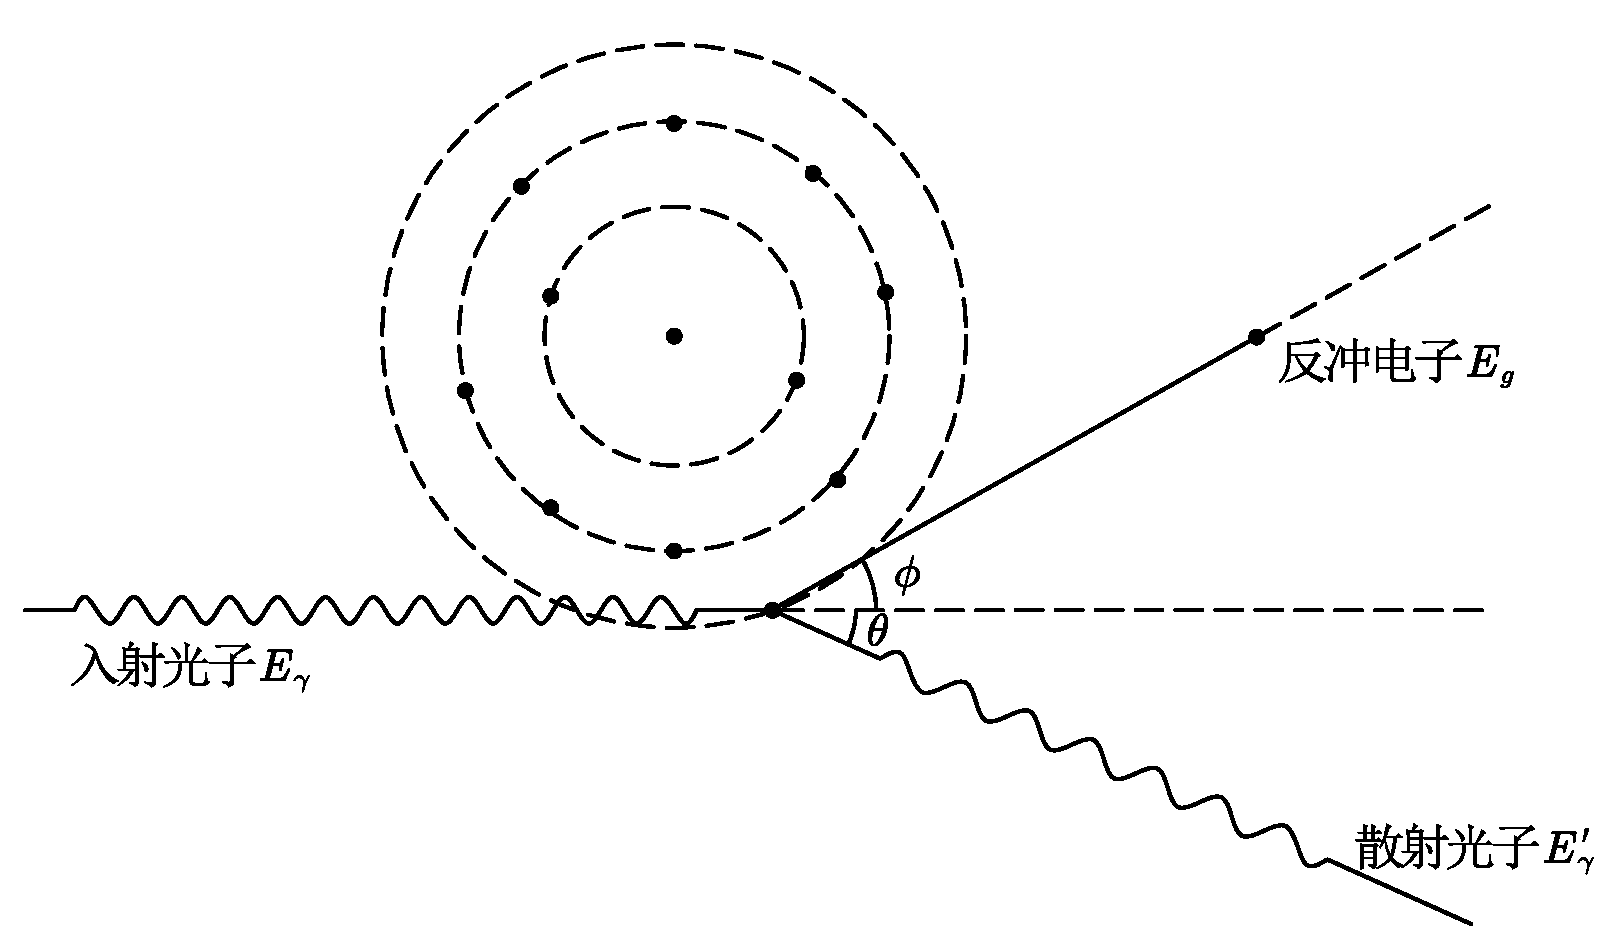
\includegraphics[width=11.5cm]{./figures/Comptn_1.pdf}
\caption{康普顿散射} \label{Comptn_fig1}
\end{figure}
由于发生康普顿散射的$\gamma$光子能量比电子的束缚能要大的多,所以$\gamma$光子与原子中的电子相互作用时,可以把电子的束缚能忽略,看成是自由电子,并视为散射发生以前电子是静止的,动能为$0$,只有静止能$m_0c^2$.散射后,电子获得速度$v$,此时电子的能量
\begin{equation}
E=\frac{m_{0} c^{2}}{\sqrt{1-\beta^{2}}}
\end{equation}
动量为
\begin{equation}
m v=\frac{m_{0} v}{\sqrt{1-\beta^{2}}}
\end{equation}
其中$\beta=v/c$,$c$为光速.

由相对论的能量和动量守恒定律可以得到:
\begin{equation} \label{Comptn_eq1}
\begin{cases}
m_{0} c^{2}+h \nu&=\dfrac{m_{0} c^{2}}{\sqrt{1-\beta^{2}}}+h \nu^{\prime} \\
\dfrac{h \nu}{c}&=\dfrac{h \nu^{\prime}}{c} \cos \theta+\dfrac{m_{0} v}{\sqrt{1-\beta^{2}}} \cos \phi \\
\dfrac{h \nu^{\prime}}{c} \sin \theta&=\dfrac{m_{0} v}{\sqrt{1-\beta^{2}}} \sin \theta
\end{cases}
\end{equation}

解方程\autoref{Comptn_eq1},可得
\begin{equation}
h \nu^{\prime}=\frac{h \nu}{1+\frac{h \nu}{m_{0} c^{2}}(1-\cos \theta)}
\end{equation}
其中$h\nu / c$是入射光子的动量,$h\nu' / c$是散射光子的动量,此式表示散射光子能量与入射光子能量及散射角的关系.